\chapter{Serwer}
\label{chap:server}

    Niniejszy rozdział przedstawia zagadnienia związane z procesem implementacji części serwerowej systemu. Uzasadnia wybór wykorzystanych technologii sprzętowych i ukazuje przepływ sterowania zarówno oprogramowania autoryzującego, jak i zarządzającego.

    Założeniem tej części procesu implementacyjnego nie było stworzenie skomplikowanego oprogramowania klasy biznesowej umożliwiającego zaawansowaną konfigurację systemu, lecz w pełni funkcjonalnego prototypu na potrzeby demonstracyjne. Wymienione technologie są wystarczające na potrzeby aplikacji prototypowych, jednak w przypadku chęci rozwijania systemu dla środowisk produkcyjnych konieczne mogłoby okazać się przemyślenie zestawu technologii w celu optymalizacji wydajności oraz zwiększenia bezpieczeństwa systemu.

    \section{Oprogramowanie autoryzujące}
    \label{s:auth_subs}

    	Zadania należące do oprogramowania autoryzującego to komunikacja z klientami oraz interakcja z bazą danych. Niewielka liczba jego funkcji powoduje, że kluczową cechą na którą zwrócono uwagę przy wyborze technologii jego implementacji jest prostota i zdolność do szybkiego stworzenia funkcjonalnego prototypu. Istotnym wymaganiem była także możliwość przeprowadzania nieskomplikowanych operacji na bazie danych.
    	Do implementacji części autoryzacyjnej serwera wybrano język Python ze względu na jego przenośność, prostą składnię oraz wbudowaną możliwość integracji z bazą danych.

    	Oprogramowanie autoryzujące składa się z pojedynczego skryptu. Jego działanie opiera się na nieskończonej pętli oczekiwania na połączenie od urządzenia klienckiego. Schemat blokowy oprogramowania autoryzującego przedstawia rysunek \ref{fig:flowchart5}.

    	\begin{figure}[]
            \centering
            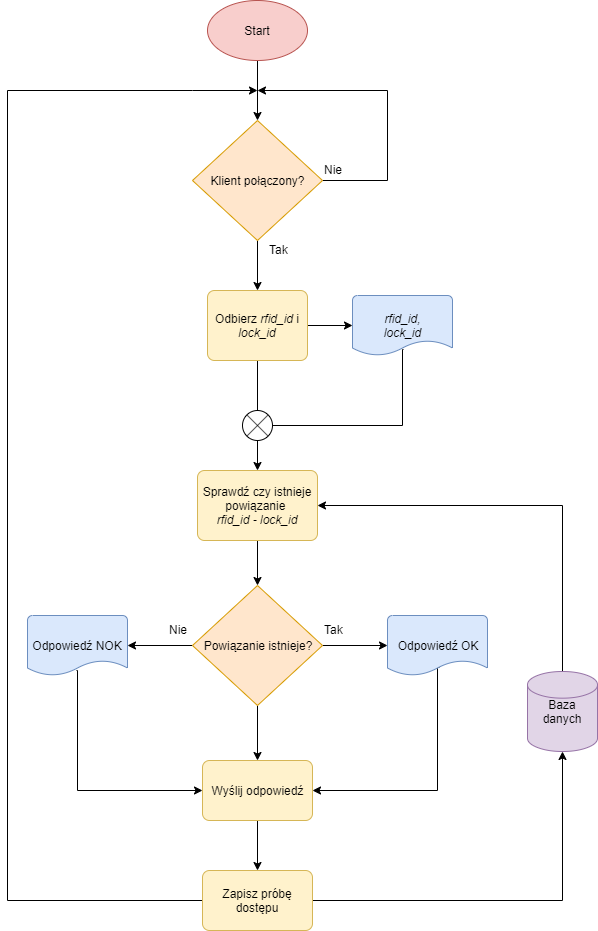
\includegraphics[width=0.85\textwidth]{chapters/images/flowchart5.png}
            \caption{Schemat blokowy przepływu sterowania oprogramowania autoryzującego}
            \label{fig:flowchart5}
        \end{figure}

    	W celu realizacji komunikacji z wykorzystaniem protokołu TLS użyto biblioteki ssl języka Python bazującej na OpenSSL. Uwierzytelnienie klienta zostało osiągnięte poprzez odpowiednią konfigurację kontekstu SSl, tak aby tryb weryfikacji wymagał poświadczenia tożsamości klienta w formie odpowiedniego certyfikatu.

    \section{Oprogramowanie zarządzające}

    	Oprogramowanie zostało podzielone na dwie współpracujące ze sobą aplikacje:

    	\begin{itemize}
    		\item Aplikacja GUI (frontend)

    			Odpowiada za prezentację danych użytkownikowi, tłumaczenie jego akcji przeprowadzanych na graficznym interfejsie na żądania HTTP i wysyłanie ich do aplikacji API.

    		\item Aplikacja API (backend)

    			Udostępnia zasoby dla aplikacji GUI. Odpowiada za odbieranie od niej żądań HTTP, przetwarzanie ich i zwracanie stosownych odpowiedzi. Zawiera większą część logiki biznesowej oraz logikę zarządzania i dostępu do danych.
    	\end{itemize}

    	Warstwową budowę oprogramowania zarządzającego przedstawia rysunek \ref{fig:mngmt_subs_layers}.

        \begin{figure}[]
            \centering
            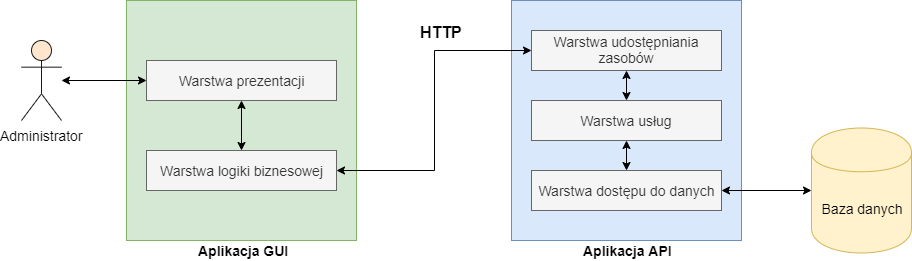
\includegraphics[width=\textwidth]{chapters/images/mngmt_subsystem_layers.png}
            \caption{Warstwowa budowa oprogramowania zarządzającego}
            \label{fig:mngmt_subs_layers}
        \end{figure}

       	Istotnym czynnikiem motywującym wybór technologii aplikacji była prostota oraz łatwość implementacji oraz rozwoju funkcjonalnej i estetycznej aplikacji demonstracyjnej zarówno po stronie przeglądarki jak i serwera. Ważną cechą była także łatwość integracji rozwiązania z bazą danych.

		Jako język implementacji aplikacji API wybrano język Python z framework'iem Flask. Ważną cechą języka Python jest wbudowane wsparcie dla bazy danych SQLite (patrz \ref{s:db}). Framework Flask jest lekką platformą do tworzenia aplikacji internetowych. Zawiera deweloperski serwer WWW, co znacznie ułatwia wytwarzanie i testowanie aplikacji.

		Do implementacji aplikacji GUI zdecydowano się na framework Angular. Angular jest otwartą platformą do tworzenia tzw. SPA (ang. \textit{Single Page Applications}). SPA to aplikacje internetowe, w których nawigacja polega na dynamicznym ładowaniu poszczególnych elementów strony zamiast pobierania całych stron z serwera. Angular napisany jest w języku TypeScript, który jest otwartoźródłowym, typowanym nadzbiorem języka JavaScript. Angular CLI jest z kolei narzędziem wspierającym pracę z framework'iem Angular poprzez udostępnienie zestawu prostych komend ułatwiających wykonywanie operacji związanych z procesem rozwijania aplikacji, takich jak tworzenie projektu, generowanie kodu źródłowego czy testowanie z użyciem wbudowanego serwera.

		Zrzuty ekranu aplikacji GUI przedstawiono na rysunkach. Są to widok tabeli identyfikatorów RFID (\ref{fig:ss1}), widok okna dodawania nowego identyfikatora (\ref{fig:ss2}) oraz widok tabeli zawierającej historię prób dostępu (\ref{fig:ss3}).

		\begin{figure}[]
            \centering
            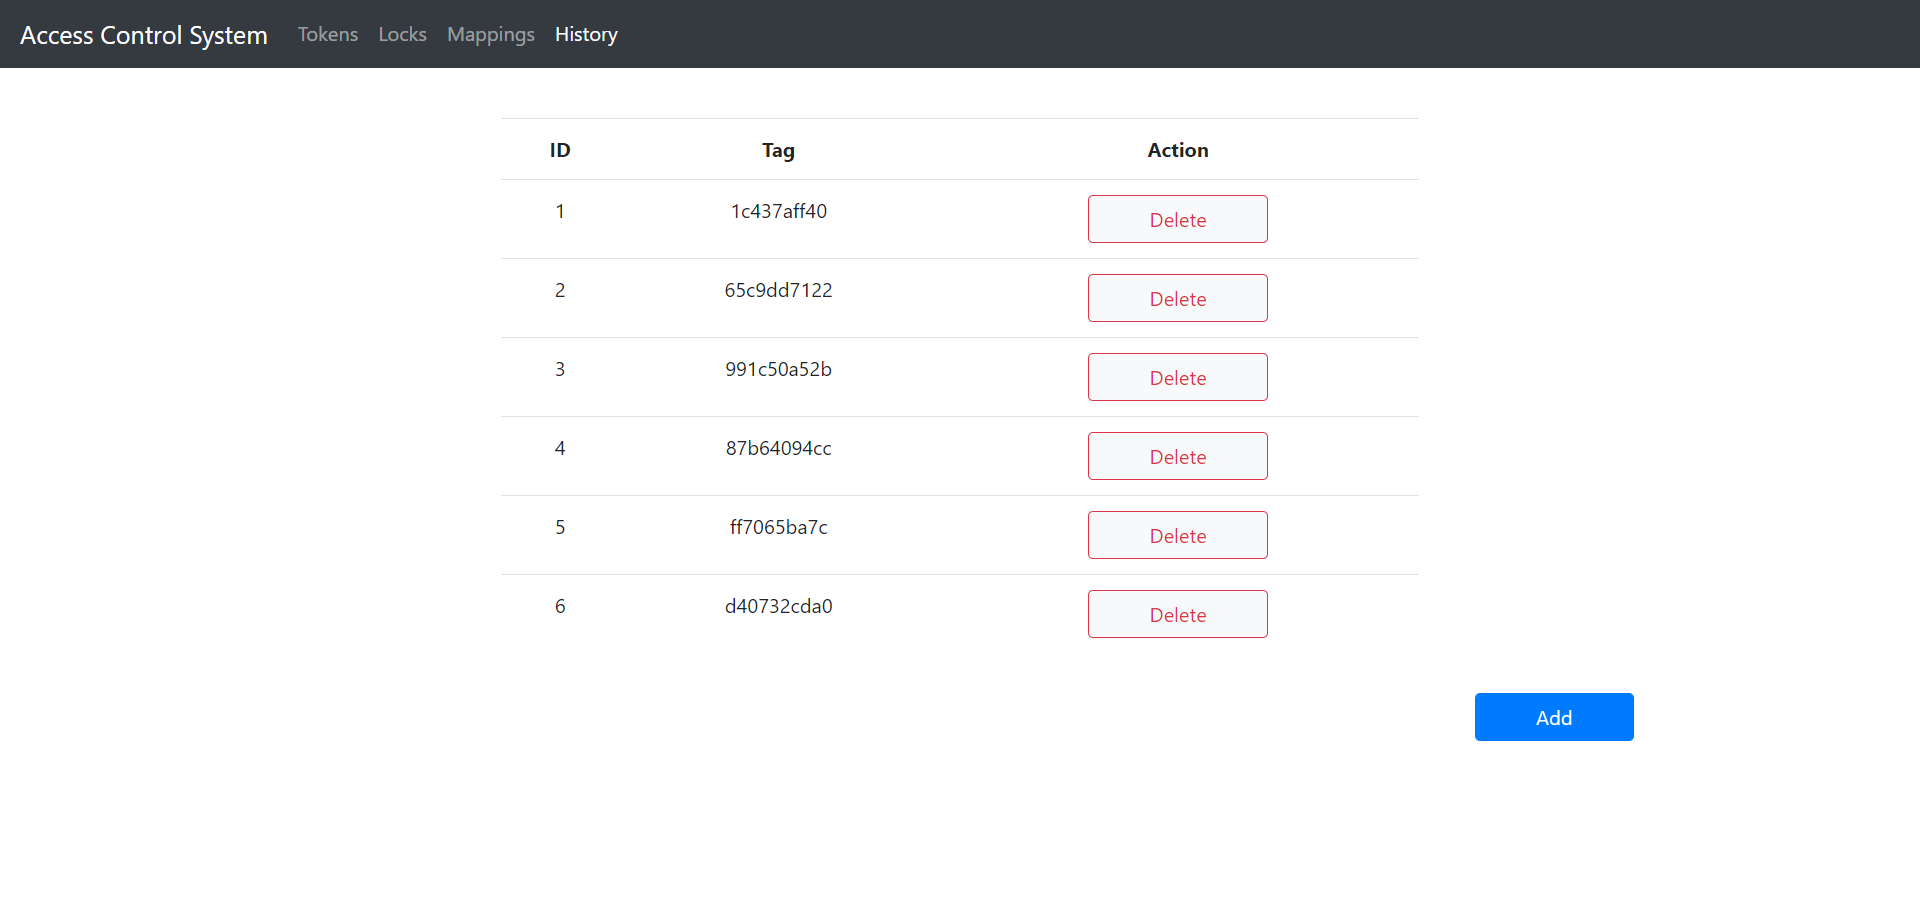
\includegraphics[width=\textwidth, frame]{chapters/images/ss1.png}
            \caption{Zrzut ekranu widoku tabeli identyfikatorów RFID}
            \label{fig:ss1}
        \end{figure}

        \begin{figure}[]
            \centering
            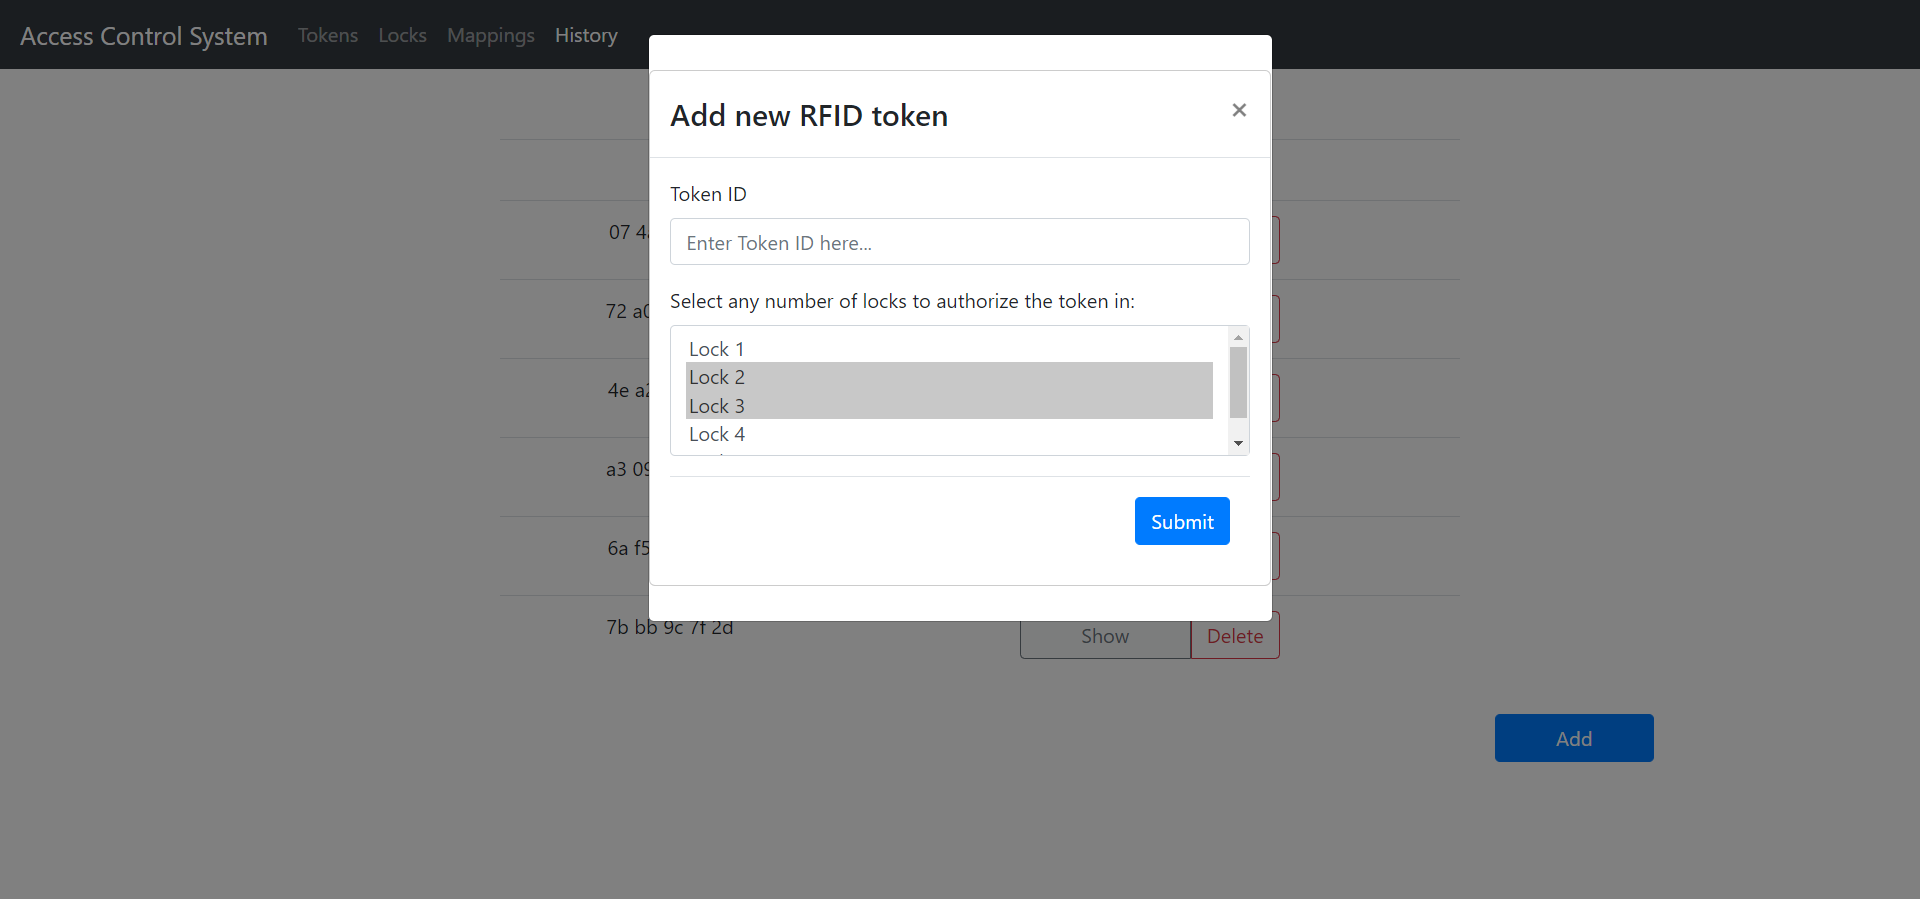
\includegraphics[width=\textwidth]{chapters/images/ss2.png}
            \caption{Zrzut ekranu widoku okna dodawania nowego identyfikatora}
            \label{fig:ss2}
        \end{figure}

        \begin{figure}[]
            \centering
            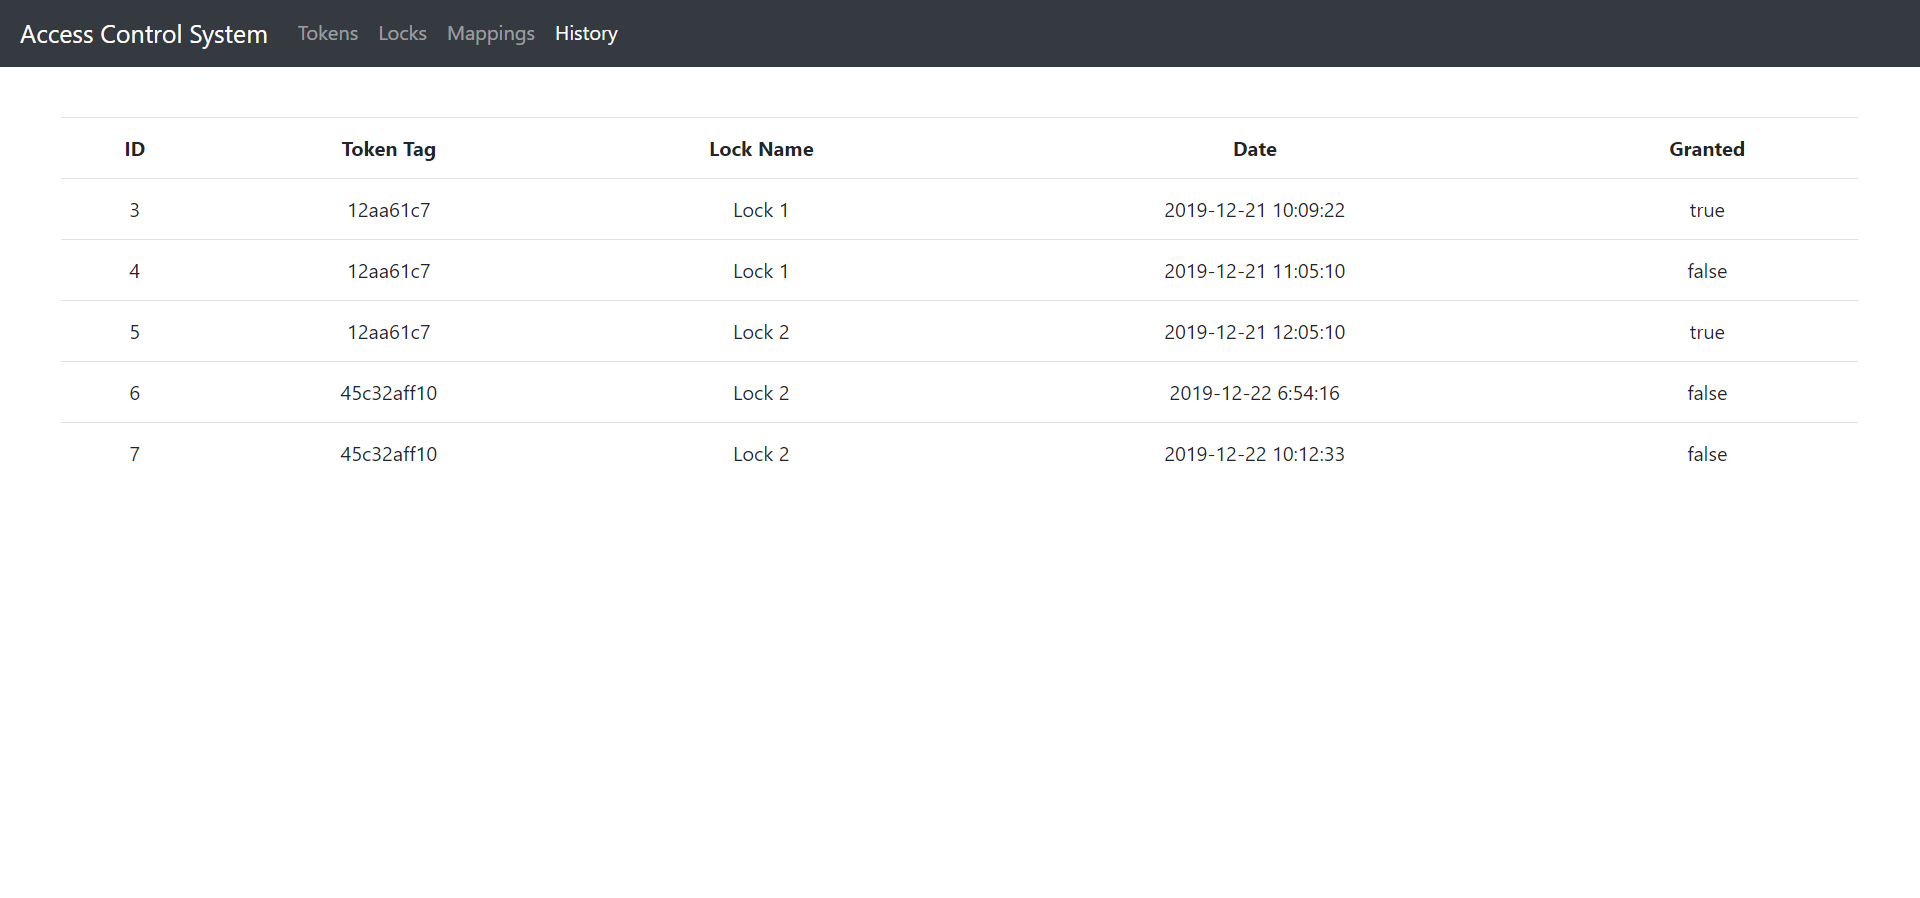
\includegraphics[width=\textwidth, frame]{chapters/images/ss3.png}
            \caption{Zrzut ekranu widoku tabeli historii prób dostępu}
            \label{fig:ss3}
        \end{figure}

    \section{Baza danych}
    \label{s:db}

    	Istotnym kryterium przydatności systemu zarządzania bazą danych była lekkość i łatwość obsługi z poziomu aplikacji internetowej napisanej w języku Python. Z tego względu zdecydowano się na system SQLite. Jest to system zarządzania bazą danych oraz biblioteka języka C implementująca taki system, obsługująca język SQL (ang. \textit{Structured Query Language}). Posiada API do wielu języków, w tym Pythona. Zawartość bazy danych przechowywana jest w pojedynczym pliku na dysku. Wszystkie powyższe cechy czynią SQLite rozwiązaniem przydatnym w szeroko pojętym procesie prototypowania.

    	Baza danych systemu tworzona jest przez aplikację API po jej uruchomieniu. Krok ten jest pomijany, jeżeli baza danych już istnieje.
